\section{实验结果与分析}
\subsection{Cache仿真结果分析}
\subparagraph{仿真代码设计}
为了实现Cache正确性的仿真验证,本次实验采用了对Cache和CMU模块的单独仿真。仿真代码的设计如下:
\begin{lstlisting}[language=Verilog]
    module cmu_sim (
        input wire clk,
        input wire rst,
        output reg [7:0] clk_count = 0,
        output reg [7:0] inst_count = 0,
        output reg [7:0] hit_count = 0
        );
        
        // instruction
        reg [3:0] index = 0;
        wire valid;
        wire write;
        wire [31:0] addr;
        wire [2:0] u_b_h_w;
        wire stall;
        inst INST (
            .clk(clk),
            .rst(rst),
            .index(index),
            .valid(valid),
            .write(write),
            .addr(addr),
            .u_b_h_w(u_b_h_w)
        );
    
        always @(posedge clk) begin
            if (rst)
                index <= 0;
            else if (valid && ~stall)
                index <= index + 1'h1;
        end
        // ram
        wire mem_cs;
        wire mem_we;
        wire [31:0] mem_addr;
        wire [31:0] mem_din;
        wire [31:0] mem_dout;
        wire mem_ack;
        data_ram RAM (
            .clk(clk),
            .rst(rst),
            .addr({21'b0, mem_addr[10:0]}),
            .cs(mem_cs),
            .we(mem_we),
            .din(mem_din),
            .dout(mem_dout),
            .stall(),
            .ack(mem_ack),
            .ram_state()
        );
        
        // cache
        wire [31:0] data_r;
        cmu CMU (
            .clk(clk),
            .rst(rst),
            .addr_rw(addr),
            .u_b_h_w(u_b_h_w),
            .en_r(~write),
            .data_r(data_r),
            .en_w(write),
            .data_w({16'h5678, clk_count, inst_count}),
            .stall(stall),
            .mem_cs_o(mem_cs),
            .mem_we_o(mem_we),
            .mem_addr_o(mem_addr),
            .mem_data_i(mem_dout),
            .mem_data_o(mem_din),
            .mem_ack_i(mem_ack),
            .cmu_state()
        );
    
        // counter
        reg stall_prev;
        
        always @(posedge clk) begin
            if (rst)
                stall_prev <= 0;
            else
                stall_prev <= stall;
        end
        
        always @(posedge clk) begin
            if (rst) begin
                clk_count <= 0;   // 时钟计数
                inst_count <= 0;  // 指令计数
                hit_count <= 0;   // 命中计数
            end
            else if (valid) begin
                clk_count <= clk_count + 1'h1;
                inst_count <= index + 1'h1;
                if (~stall_prev && ~stall)
                    hit_count <= hit_count + 1'h1;
            end
        end
    
    endmodule    
\end{lstlisting}

为了验证结果,本次实验还设计了一个单独的Test Bench以供测试:
\begin{lstlisting}[language=verilog]
module inst (
    input wire clk,
    input wire rst,
    input wire [3:0] index,  // instruction index
    output wire valid,  // stop running if valid is 0
    output wire write,  // write enable signal for cache
    output wire [31:0] addr,  // address for cache
    output wire [2:0] u_b_h_w
    );
    reg [39:0] data [0:9];
    initial begin
        data[0] = 40'h0_2_00000004;  // read miss               1+17
        data[1] = 40'h0_3_00000019;  // write miss              1+17
        data[2] = 40'h1_2_00000008;  // read hit                1
        data[3] = 40'h1_3_00000014;  // write hit               1
        
        data[4] = 40'h2_2_00000204;  // read miss               1+17
        data[5] = 40'h2_3_00000218;  // write miss              1+17
        data[6] = 40'h0_3_00000208;  // write hit               1
        data[7] = 40'h4_2_00000414;  // read miss + dirty       1+17+17
        data[8] = 40'h1_3_00000404;  // write miss + clean      1+17
        data[9] = 40'h0;           // end                     total: 128
    end
    assign
        u_b_h_w = data[index][38:36],
        valid = data[index][33],
        write = data[index][32],
        addr = data[index][31:0];
        
endmodule
\end{lstlisting}

\subparagraph{仿真结果分析}
根据上述仿真代码,实验的仿真结果如下,在此部分我组将对仿真结果进行逐一分析。
首先同样是多周期的重置过程,以保证cache与内存内容的彻底重置。
\begin{figure}[H] %H为当前位置,!htb为忽略美学标准,htbp为浮动图形
	\centering %图片居中
	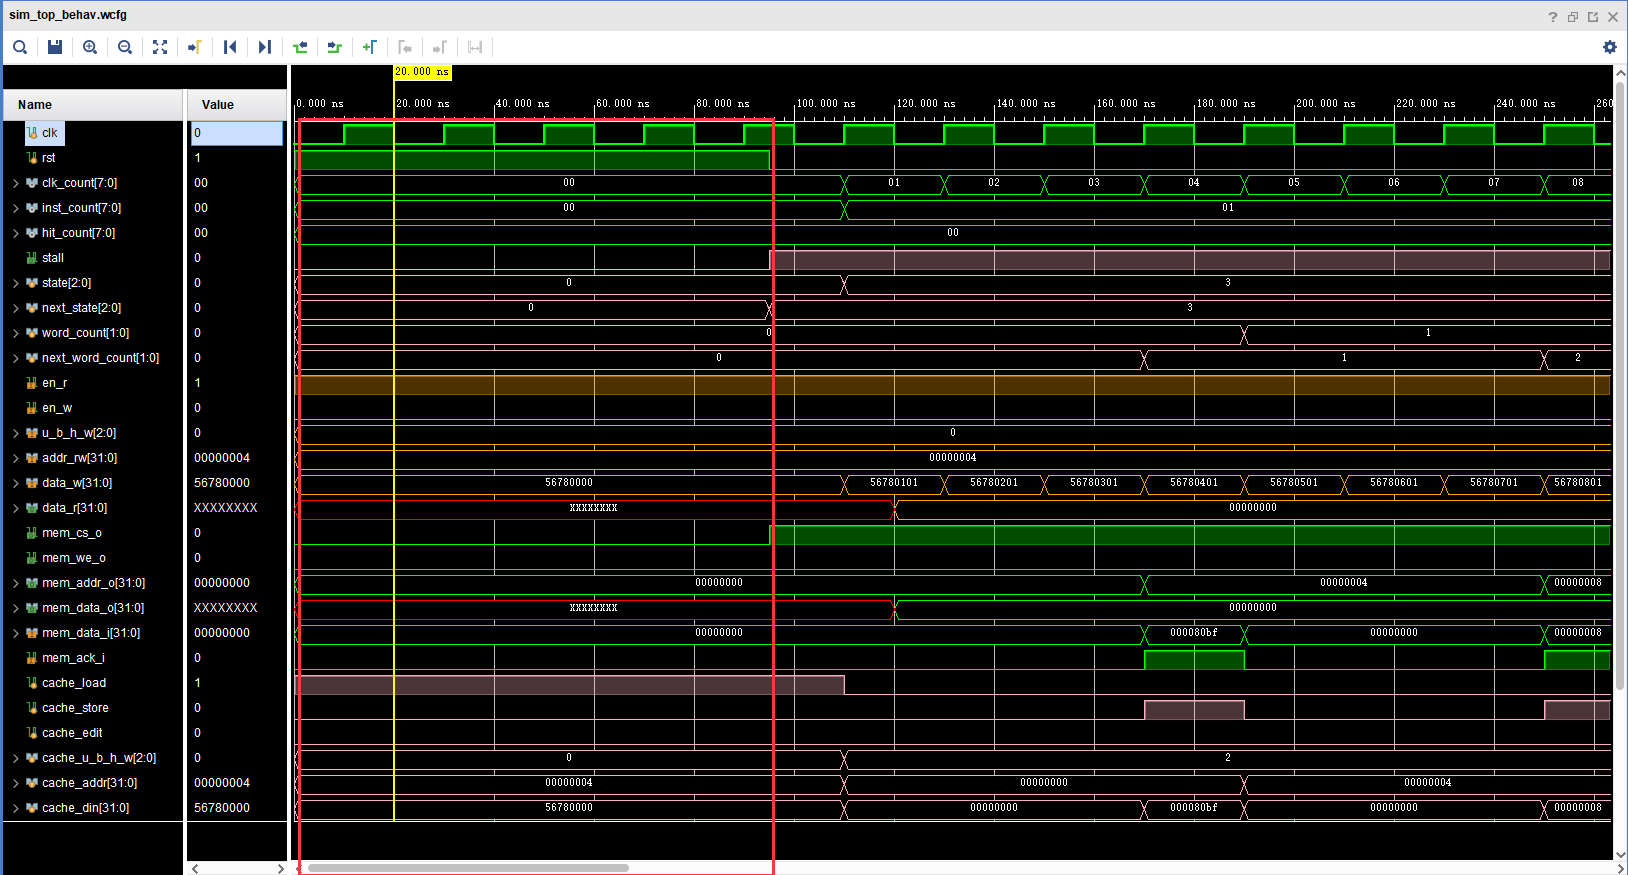
\includegraphics[width=1.0\textwidth]{figs/sres1.png} %插入图片,[]中设置图片大小,{}中是图片文件名
	\caption{重置过程} %最终文档中希望显示的图片标题
	\label{Fig.4} %用于文内引用的标签
\end{figure}